\documentclass[11pt]{article}
\usepackage[]{babel}
\usepackage{natbib}
\usepackage{url}
\usepackage[utf8x]{inputenc}
\usepackage{amsmath}
\DeclareMathOperator*{\argmax}{argmax} % thin space, limits underneath in displays
\DeclareMathOperator*{\argmin}{argmin} % thin space, limits underneath in displays
\usepackage{graphicx}
\graphicspath{{images/}}
\usepackage{parskip}
\usepackage{fancyhdr}
\usepackage{vmargin}
\usepackage{breqn} % Automatic equation breaker
\usepackage{amssymb} %% <- for \square and \blacksquare
\usepackage{breqn} % used for automatic equation breaking
\newcommand{\QEDA}{\null\nobreak\hfill\ensuremath{\blacksquare}}%
\newcommand{\QEDB}{\null\nobreak\hfill\ensuremath{\square}}%
\newcommand{\smallspace}{\hspace{0.5cm}}
\setcounter{secnumdepth}{0} % for avoiding the numbering
\usepackage{hyperref} % to click and go to pointed place in the document
\usepackage{tcolorbox} % if we want to use the boxes
\usepackage{cancel} % for cool cancellations
\newenvironment{sfemph}{\begin{sffamily}\begin{emph}}{\end{sffamily}\end{emph}}
 % the text inside the exercise setup will be emphasized
\usepackage{xcolor} % Colored text
\usepackage{minted} % For highlighting Python code
\usepackage[ruled,vlined]{algorithm2e} % for algorithms
\usepackage{biblatex} % bibliography
\addbibresource{references.bib}

% Set defaults for minted
\setminted{frame=lines,
framesep=2mm,
baselinestretch=1.2,
bgcolor=,
fontsize=\footnotesize,
linenos
}
\usepackage{comment} %for multiline commenting



%%%%%%%%%%%%%%%%%%%%%%%%%%%%%%%%%%%%%%%%%%%%%%%%%%%%%%%%%%%%%%%%%%%%%%%%%%%%%%%%%%%%%%%%%
% MODIFY KAIST TEMPLATE DATA HERE

\title{Studies on Model-Free Control of Dynamical Systems with Visual Feedback}							
\author{Federico Berto}							
\date{\today}											
\newcommand{\professor}{***} 
\newcommand{\studentid}{***} 
\newcommand{\coursename}{Optimal Control}
\newcommand{\courseid}{***}
%%%%%%%%%%%%%%%%%%%%%%%%%%%%%%%%%%%%%%%%%%%%%%%%%%%%%%%%%%%%%%%%%%%%%%%%%%%%%%%%%%%%%%%%%

%%%%%%%%%%%%%%%%%%%%%%%%%%%%%%%%%%%%%%%%
\setmarginsrb{3 cm}{2.5 cm}{3 cm}{2.5 cm}{1 cm}{1.5 cm}{1 cm}{1.5 cm}

\makeatletter
\let\thetitle\@title
\let\theauthor\@author
\let\thedate\@date
\makeatother

\pagestyle{fancy}
\fancyhf{}
\renewcommand{\headrulewidth}{0.4pt}% Default \headrulewidth is 0.4pt
%\renewcommand{\footrulewidth}{0.4pt}% Default \footrulewidth is 0pt
\rhead{\theauthor}
%\rhead{\includegraphics[width=1cm]{example-image-a}}
\lhead{Optimal Control Report}
\chead{\raisebox{-1ex}{
\includegraphics[width = 3cm, shift down = 1cm]{kaist.png}}}
\cfoot{Page \thepage}

\begin{document}

%%%%%%%%%%%%%%%%%%%%%%%%%%%%%%%%%%%%%%%%%%%%%%%%%%%%%%%%%%%%%%%%%%%%%%%%%%%%%%%%%%%%%%%%%

\begin{titlepage}
	\centering
    \textsc{\LARGE  Korea Advanced Institute of Science \\ \smallskip and Technology}\\[1 cm]	% University Name
    
\includegraphics[scale = 0.18]{kaist_round_logo.png}\\[1.5 cm]	% University Logo
	\textsc{\Large \coursename}\\[0.5 cm]				% Course Code
	\rule{\linewidth}{0.2 mm} \\[0.4 cm]
	{ \huge \bfseries {\thetitle}}\\
	\rule{\linewidth}{0.2 mm} \\[1.5 cm]
	

	\begin{minipage}{0.5\textwidth}
		\begin{flushleft} \large
			\emph{Professor:}\\
		    \professor \\ [0.5cm]
            \emph{Course ID:}\\
            \courseid
			\end{flushleft}
			\end{minipage}~
			\begin{minipage}{0.4\textwidth}
            
			\begin{flushright} \large
			\emph{Student:} \\
			\theauthor \\[0.5cm]
			\emph{ID number:}\\
			\studentid \\
		\end{flushright}
        
	\end{minipage}\\[2 cm]
	
	
    %\thedate

    
	
\end{titlepage}

% %%%%%%%%%%%%%%%%%%%%%%%%%%%%%%%%%%%%%%%%%%%%%%%%%%%%%%%%%%%%%%%%%%%%%%%%%%%%%%%%%%%%%%%%%

% %%%%%%%%%%%%%%%%%%%%%%%%%%%%%%%%%%%%%%%%%%%%%%%%%%%%%%%%%%%%%%%%%%%%%%%%%%%%%%%%%%%%%%%%%
\begin{abstract}
    Modeling is well know to be one of the most difficult challenges when developing control systems: partial observability and disturbances in the control system can make the system unstable; especially considering the cases of complex and nonlinear ones. Model-free control is an alternative for solving control problems without the need to design a complex model in the first place: in particular, Reinforcement Learning has shown promising results in controlling nonlinear systems even when the state variables cannot be derived directly, such as in the case of a system in which sensors are unavailable or broken. The goal of this report is to demonstrate the ability of Deep Q-Network algorithm in controlling a dynamical system with the aim of stabilizing an inverted pendulum using only raw pixels as state feedback: this model-free formulation does not require any assumption or previous knowledge of the dynamical system unlike most controllers.
    
\end{abstract}

    
\section{Introduction}

Reinforcement Learning \cite{sutton1998introduction} is one of the branches of Machine Learning which has seen a surge in interest in recent years because of its ability to handle complex tasks with minimal human intervention and, in the case of model-free reinforcement learning, to learn a representation of the state-action space without needing the actual space variables.\\
Reinforcement Learning (RL) has been successfully used for playing complex Atari games \cite{mnih2013playing}, for mastering the game of GO \cite{Silver_2016} and even Starcraft II \cite{Starcraft}, showing important results regarding high-dimensional state-action spaces.\\
Another interesting application is the model-free control, which is still an open research topic \cite{DBLP:journals/corr/abs-1912-03513} given the complex nature of the continuous state: we will explore this setup in the report and show its promising capabilities in handling non-linear systems without the need of an explicit model formulation, unlike many controllers do. \\
Moreover, we will show that the performance of the controller is better, to the best of the author's knowledge, than other similar setups of the raw-pixels based inverted pendulum thanks to some tweaks we will explore.

\section{Brief Overview of Reinforcement Learning}
The control system can be defined as in the Figure \ref{fig:agentenvironment}, usually called the \textit{agent-environment interface}, which is the correspondent of the controller-plant interface in classical control. This framework can be defined by the following:

\begin{figure}[h]
	\centering
	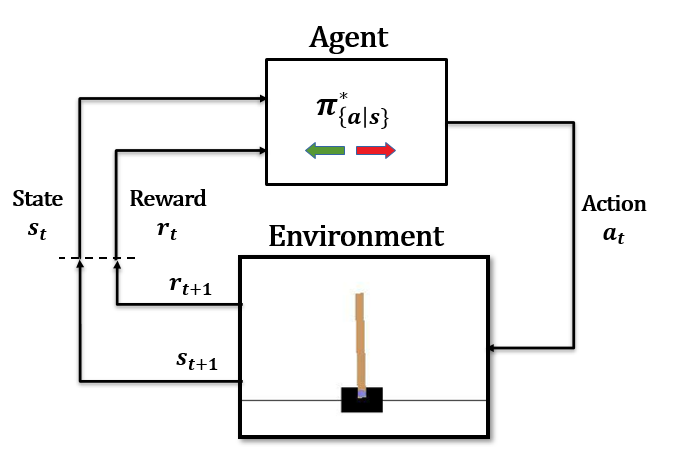
\includegraphics[width=12cm]{agent-environment.png}
	\caption{Agent-Environment interface for the inverted pendulum system. $\pi^*_{ \{ a \mid s \} }$ denotes the optimal policy}
	\label{fig:agentenvironment}
\end{figure}

\begin{itemize}
	\item \textit{Policy}: set of \textit{actions} (which are the control inputs in the Optimal Control field) to be selected given the current state.
	\item \textit{Reward}: a scalar value to be maximized by the agent. This value is another feedback along with the state at each time step; this is usually set as a positive number if the agent is performing as desired and as a negative number otherwise. In the Optimal Control terms, it is equivalent to the opposite of the cost function.
	\item \textit{Value function}: whereas the reward defines what is good in a short time, the value function defines what is good in the long run; it is defined as the sum of the discounted future rewards that can be accumulated from a particular state.
\end{itemize}

The goal of the control system (agent) is to maximize the cumulative discounted reward defined as following from the environment:

\begin{equation}
	G_t  =  R_{t+1} + \gamma R_{t+2} + ...  =  \sum_{k=0}^{\infty}\gamma^k R_{t+k+1}
\end{equation}
where $\gamma \in [0,1]$ is a discount factor used for giving a lighter weight to far-away future rewards. \\
The policy $\pi$ choosing the actions leading to the highest reward can be chosen for the Deep Q-Networks in the \textit{$\varepsilon$-greedy} way:
\begin{equation}
\pi(a|s) = \begin{cases}
1 - \varepsilon, & \text{if $a = \argmax_{a \in \mathcal{A}} \, q^*(s,a)$}\\
\varepsilon, & \text{a random action}.
\end{cases}
\end{equation}
where $q^*(s,a)$ denotes the \textit{state-action value} and $\varepsilon$ is chosen depending on how much \textit{exploration} (randomly trying new actions for finding out undiscovered and possibly better states and actions) and \textit{exploitation} (choosing the known best action) ration we want the system to have.

\paragraph{Trajectories of the system}
In order to optimize the system, we need to know what trajectories lead to the best cumulative reward. In this setup, \textit{agent} is the entity acting on the \textit{environment}, that given a $state \ S_t \in \mathcal{S}$ selects one or more $actions \ A_t \in \mathcal{A}$ for interacting with the environment. Our agent then gets feedback from the environment itself: it gets a scalar valued $reward \ R_{t+1} \in \mathcal{R}$, and gets in a new state $S_{t+1} \in \mathcal{S}$. In a \textit{finite} Markov Decision Process the set of states, actions and rewards ($\mathcal{S},\mathcal{A},\mathcal{R})$ contains a finite number of elements; nonetheless, the problem can be extended in the continuous case. The agent-environment feedback loop repeats over time and it is updated at each time \textit{step}: action selection, state and reward signals are sent only at specific moments in time (t = 0,1,2,3...). The sequence of actions, states and rewards defines a \textit{trajectory} in time that can be described as: 
\begin{equation}
	S_0, A_0, R_1, S_1, A_1, R_2, S_2, A_2, R_3... 
\end{equation}
This sequence can be used on the go for optimizing the system or stored in a buffer and used later in randomized batches allowing for better stability of the training.


\section{Experimental Setup}

We will conduct the experiments with the inverted pendulum simulation from OpenAI Gym \cite{brockman2016openai}. Also known as the \textit{cart-pole}, the inverted pendulum is a common benchmark for testing control systems because of its relative simplicity and yet challenging feat because of the system's nonlinearities. This system can be controlled with well-known controllers, such as the Linear Quadratic Regulator for the linearized version, or with i.e. the Model Predictive Control for the non-linear version, such as for the pendulum swing up; however, our task is more challenging because of the absence of the system's model.

\begin{table}
	\centering
	\begin{tabular}{ |p{2cm}|p{4cm}|p{2cm}|p{2cm}|  }
		\hline
		\multicolumn{4}{|c|}{Observation Space} \\
		\hline
		Num & Observation & Min & Max \\
		\hline
		0 & Cart Position & -2.4 & 2.4 \\
		1 & Cart Velocity & $-\infty$ & $+\infty$ \\
		2 & Pole Angle & $\-41.8$\textdegree & $41.8$\textdegree \\
		3 & Pole Angular Velocity & $-\infty$ & $\infty$ \\
		\hline
	\end{tabular}
	\label{table:tableenvironment}
	\caption{Inverted Pendulum's observation space}
\end{table}

\paragraph{The observations space} The simulation is made of a four dimensional observation space of the cart position, cart velocity, pole angle, and pole angular velocity as shown in Table \ref{table:tableenvironment}.

 The available actions are two discrete ones: push a cart left or right. The reward is defined as +1 for every time step the inverted pendulum stands including the termination step. The task is considered achieved when the average reward of the last 100 episodes reaches a score close to the maximum score of 200. Episode termination occurs when:

\begin{itemize}
	\item The pole angle is more than $\pm 12$\textdegree
	\item The cart position is more than $\pm 2.4$ (i.e. the center of the cart almost reaches the edge of the display)
	\item The episode length is greater than 200
  \end{itemize}

Although the observation space is fixed for the simulation, our vision-based control is based on a set of images of the simulation, which significantly increase the state observation size. In order to let the algorithm derive a good approximation of the state, we will use a sequence of the last $N$ images (i.e., the last 2 frames) for making it capable to infer the dynamics of the pendulum.

\paragraph{The Algorithm: Deep Q-Learning}

The Deep Q-Learning algorithm has shown state-of-the-art performance in multiple frameworks, such as the Atari framework \cite{mnih2013playing}. 
In order to approximate the action-value function,  we will employ a Convolutional Neural Network $Q(s,a; \theta) \approx Q^*(s,a)$. For our purposes, $\theta$ will denote the set of weights of the network, which we will refer to as Q-network. A Q-network can be trained by minimizing a sequence of loss functions $L_i(\theta_i)$ changing at each iteration i,

\begin{equation}
	L_i(\theta_i) = \mathbb{E}_{s,a \sim \rho(\cdot)}[\left(y_i - Q(s,a;\theta_i)\right)^2],
	\label{eq:lossfunction}
\end{equation}

where $y_i = \mathbb{E}_{s' \sim \mathcal{E}} [r + \gamma \max_{a'}Q(s', \theta_{i-1}) | s,a]$ is the target for iteration $i$, $\rho(s,a)$ is a probability distribution over sequences $s$ and actions $a$. The parameters from the previous iteration $\theta_{i-1}$ are kept fixed when optimizing the loss function $L_i(\theta_i)$. The targets depend on the network weights: for this reason, it differs from classical weights used in supervised learning, which are fixed before learning itself begins. 
\medskip

\indent Since we want to minimize the loss function for obtaining a better fit of the networks with respect to the real action value function, we want to compute the gradient with respect to the weights:

\begin{equation}
	\nabla_{\theta_i}L_i (\theta_i) = \mathbb{E}_{s,a \sim \rho(\cdot); s' \sim \mathcal(E)} [(r + \gamma \max_{a'} Q (s', a'; \theta_{i-1}) -  Q(s,a; \theta_i)) \nabla_{\theta_i} Q(s,a; \theta_i)]
	\label{eq:gradientloss}
\end{equation}

The loss function is then minimized by either using stochastic gradient descent or more sophisticated methods like RMSprop. The behavior policy is $\epsilon$-greedy for ensuring sufficient exploration.
\medskip 

\indent What makes the algorithm work is a technique known as \textit{experience replay}\cite{schaul2015prioritized}, by which we store the agent's experiences (also referred to as transitions) at each time-step, $e_t = (s_t, a_t, r_t, s_{t+1})$, in a data set $ \mathcal{D} = (e_1, ..., e_N)$, pooled over many episodes into a \textit{replay memory}. In the inner loop of our algorithm we apply Q-Learning updates, or mini-batch updates, to samples of experience, $e \sim \mathcal{D}$, picked up randomly from the pool of stored samples. After performing experience replay, the agent executes an action according to an $\epsilon$-greedy policy. Deep Q-Learning with experience replay is written in pseudo-code in Algorithm \ref{alg:DQN}.
\begin{algorithm}[h]
	\caption{Deep Q-Learning with Experience Replay}
	\label{alg:DQN}
	\SetAlgoLined
	\DontPrintSemicolon
	Initialize replay memory $\mathcal{D}$ \;
	Initialize action value function Q with random weights \;
	\Repeat{terminated}{
		Observe initial state $s_1$\;
		\For{t=1: T}{
			Select an action $a_1$ using policy derived from Q (e.g. $\epsilon$-greedy)\;
			Carry out action $a_t$\;
			Observe reward $r_t$ and new state $s_{t+1}$\;
			Store transition $(s_t, a_t, r_t, s_{t+1})$ in replay buffer $\mathcal{D}$\;
			Sample random transitions $(s_j, a_j, r_j, s_{j+1})$ from $\mathcal{D}$\;
			Calculate target for each transition \;
			% MATCH SYNTAXXX!! LIKE s'
			
			\begin{equation}
			\text{Set } y_i = \begin{cases}
			r_j & \text{if } s_{j+1} \text{ is terminal}\\
			r_j + \gamma \max_{a'} Q(s_{j+1},a';\theta) & \text{if } s_{j+1} \text{ is non-terminal}			
			\end{cases}
			\end{equation}
			
			Train the Q network on $(y_j - Q(s_j, a_j; \theta))^2$ using Equation \ref{eq:gradientloss}
		}
	}
\end{algorithm}

The following is the Python code for the experience replay, which is of paramount importance for decoupling time-dependent transitions which would introduce a bias in the system:
\begin{minted}{python}
class ReplayMemory(object):
"""Replay Memory class for storing system's trajectories"""
    def __init__(self, capacity):
        self.capacity = capacity
        self.memory = []
        self.position = 0

    def push(self, *args):
        """Saves a transition."""
        if len(self.memory) < self.capacity:
            self.memory.append(None) # if we haven't reached full 
            # capacity, we append a new transition
        self.memory[self.position] = Transition(*args)  
        self.position = (self.position + 1) % self.capacity # e.g if the capacity 
        # is 100, and our position is now 101, we don't append to position 101
        # (impossible), but to position 1 (its remainder), overwriting old data

    def sample(self, batch_size):
        return random.sample(self.memory, batch_size) 

    def __len__(self): 
        return len(self.memory)
\end{minted}
Deep Q-Learning has several advantages by using experience replay. Firstly, since each step of experience is potentially used in many weight updates, we have a greater data efficiency. Secondly, randomizing the samples allows for improved efficiency and reduces the updates variance, given that learning directly from consecutive samples of experience is inefficient due to the strong correlations between the samples. Thirdly, by learning off-policy we may be able to avoid dangerous unwanted feedback loops. For example, if we did train on-policy, if the maximizing action were to move on the left then the training samples would be dominated by samples from the left-hand side; if the maximizing action were the opposite one on the right, the same would happen with the right-hand side samples. This behavior could lead to unwanted outcomes, like getting stuck in a poor local minimum, or even catastrophically diverge. Thus, by using the off-policy experience replay we are able to smooth out learning and to avoid oscillation or divergence in the parameters.



\\
The exploration and exploitation problem is dealt with by the use of the following $\varepsilon_{threshold}$, which decays over time; a lower threshold will result in higher exploitation of the learned optimal known actions:

\begin{equation}
	\varepsilon_{threshold} = \varepsilon_{final} + (\varepsilon_{initial}-\varepsilon_{final})e^{-t/\varepsilon_{decay}}
\end{equation}

% \indent As regard the other two parameters, the \textit{kernel size} is the size of the square filter actuating convolution over the inputs (i.e. in our implementation we have a 5x5 filter). The second parameter, the \textit{stride}, is the number of pixels which are "skipped" each time while making the filter convolve. A higher stride will make the model less precise, but slower in learning; a $stride = 2$ is usually chosen because has been empirically proven to be the best choice for CNNs.


\section{Towards Vision-Based Control}

The first steps in trying to solve the inverted pendulum problem with raw pixels were based on a first implementation from Adam Paszke\footnote{\href{https://pytorch.org/tutorials/intermediate/reinforcement_q_learning.html}{Source: pytorch.org}}. The algorithm is based on Convolutional Neural Networks for predicting Q-values and implements basically the same structure of DQN.\\
Although this implementation was showing improvements in training, no matter how much training the system received, the mean reward was always swinging up and down and showing no sign of convergence or divergence. In particular, after some tenths of episodes showing an abrupt improvement in performance there were several episodes in which the agent "forgot" about the previous experiences, suddenly decreasing the performance. The problem that needs to be solved is the overfitting of the Convolutional Neural Network, which overestimated the state-action values leading to a sub-optimal policy.

\subsection{Dealing with Overfitting}

% As regards the overfitting problem there are a couple of tweaks to prevent it from happening at all. First of all, we implement a \textit{Dropout}\footnote{Dropout\cite{srivastava2014dropout} is a method by which some neural network neurons are switched off during training with a probability $p_i$, hence "dropped-out". During the testing phase, all the neurons are switched on with their output multiplied by a weight $p_i$. This method has proven to make neural networks more stable and robust.} regularization for improving the network stability. However, this has little effect in the training process, because of the intrinsic problem of learning, forgetting and learning again.
\paragraph{Improving Image Pre-Processing}
One first steps of state observation improvement implies simplifying the network by feeding it with a grayscale as input, thus reducing by one third the input dimensionality. Besides, the use of image subtraction used in the initial implementation could not capture some states; indeed, a better way to deal with changing environments over time is to feed the neural network a batch of images, them being the last N frames. This way, the state keeps track of past behaviors. By considering at least the last $N=2$ frames, velocity features can be extracted by the neural network from the image state.

\begin{figure}[h!]
	\label{fig:ExampleExtractScreen}
	\centering
	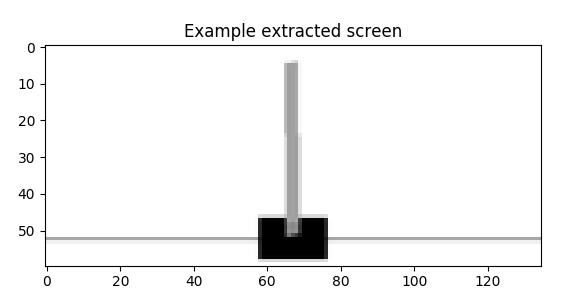
\includegraphics[width=10cm]{images/example_extracted_screen.png}
	\caption[Pre-processed image of the environment]{Extracted screen from the inverted pendulum environment: the image is extracted by cropping, downsampling and applying grayscaling}
\end{figure}

\paragraph{Early Stopping}
Thus, another method we can use is that of the \textit{Early Stopping}:  in order to prevent overfitting, the agent is trained up to a point in which it has learned optimal behavior; from that point onward it would start behaving worse and worse and then restarting learning from scratch. We can detect this optimal situation by inserting a score threshold: when the mean of the last $K$ episodes overcome this threshold $\xi$, we stop the neural networks optimization. We have empirically set these two new hyper-parameters, which can be tweaked, to $K = 20$ and $\xi= 142$.\\

\paragraph{Reward Function Design}
The reward function design is one of the most important aspects in Reinforcement Learning and can make the difference between an agent not training at all and one able to achieve super-human performance. Instead of the usual reward function from OpenAI Gym, we can build a new one being able to better give a feedback on our agent's decisions:

\begin{equation}
\label{eq:reward}
\begin{aligned}
	r_1 = \frac{x_{max} - |x|}{x_{max}} - 0.8 \\
	r_2 = \frac{\theta_{max} - |\theta|}{\theta_{max}} - 0.5 \\
	r_{tot} = r_1 + r_2 
\end{aligned}
\end{equation}
However, in this case the reward function just has a minor impact on the overall performance, so we may as well use one which doesn't explicitly employ the state variables.

\section{Final Model}
\begin{table}[h!]
	\centering
	\begin{tabular}{ |p{4cm}|p{3cm}|p{2cm}|p{1.5cm}|p{1.2cm}|  }
		\hline
		\multicolumn{5}{|c|}{Parameters} \\
		\hline
		Layer & Number of Filters/Neurons & Activation & Kernel Size & Stride \\
		\hline
		Convolutional Layer 1 & 64 & ReLu & 5 & 2\\
		\hline
		Convolutional Layer 2 & 64 & ReLu & 5 & 2 \\
		\hline
		Convolutional Layer 3 & 32 & ReLu & 5 & 2 \\
		\hline
		Linear Output Layer  & 1792 & None & - & - \\
		\hline
	\end{tabular}
	\label{table:NeuralNetwork}
	\caption{Convolutional Neural Network hyper-parameters}
\end{table}
	
After improving the model with the aforementioned techniques, we obtain the following Convolutional Neural Network described in Table \ref{table:NeuralNetwork}. As regards the loss function and optimizer, we use:
\begin{itemize}
	\item Loss Function: \textit{Huber loss function}, which is: 
	\begin{equation}
		L(Q_{target}, Q_{predicted}) = \frac{1}{2}(Q_{target}-Q_{predicted})^2
	\end{equation}
	\item Optimizer: \textit{RMSprop}, which is able to do a gradient descent of the error in almost the most optimal path
\end{itemize}

The Python code for the DQN is the following; it takes a sequence of images as input and outputs the value function corresponding to each action:
\begin{minted}{python}
class DQN(nn.Module):
"""Convolutional Neural Network predicting the state-action values"""
    def __init__(self, h, w, outputs):
        super(DQN, self).__init__()
        self.conv1 = nn.Conv2d(nn_inputs, HIDDEN_LAYER_1, 
            kernel_size=KERNEL_SIZE, stride=STRIDE) 
        self.bn1 = nn.BatchNorm2d(HIDDEN_LAYER_1)
        self.conv2 = nn.Conv2d(HIDDEN_LAYER_1, HIDDEN_LAYER_2,
            kernel_size=KERNEL_SIZE, stride=STRIDE)
        self.bn2 = nn.BatchNorm2d(HIDDEN_LAYER_2)
        self.conv3 = nn.Conv2d(HIDDEN_LAYER_2, HIDDEN_LAYER_3,
            kernel_size=KERNEL_SIZE, stride=STRIDE)
        self.bn3 = nn.BatchNorm2d(HIDDEN_LAYER_3)
        
        # Number of Linear input connections depends on output of conv2d layers
        # and therefore the input image size, so compute it.
        def conv2d_size_out(size, kernel_size = KERNEL_SIZE, stride = STRIDE):
            return (size - (kernel_size - 1) - 1) // stride  + 1
            
        convw = conv2d_size_out(conv2d_size_out(conv2d_size_out(w)))
        convh = conv2d_size_out(conv2d_size_out(conv2d_size_out(h)))
        linear_input_size = convw * convh * 32
        nn.Dropout() # Adds further regularization
        self.head = nn.Linear(linear_input_size, outputs)

    def forward(self, x):
    """Forward pass in the network"""
        x = F.relu(self.bn1(self.conv1(x)))
        x = F.relu(self.bn2(self.conv2(x)))
        x = F.relu(self.bn3(self.conv3(x)))
        return self.head(x.view(x.size(0), -1))
\end{minted}


\begin{figure}
    \centering
    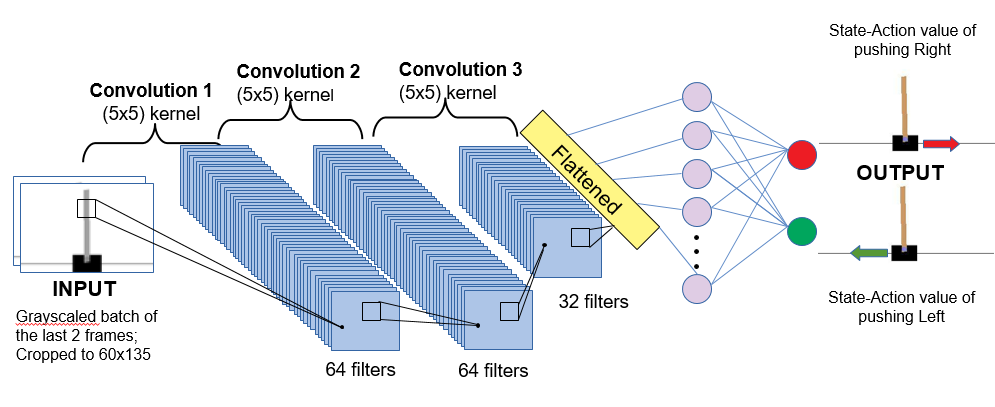
\includegraphics[width=\linewidth]{architecture.png}
    \caption{Architecture of the DQN with a Convolutional Neural Network for approximating state-action values}
    \label{fig:architecture}
\end{figure}

The final architecture of the DQN is represented in \ref{fig:architecture}. The following table shows the main Hyper-Parameters, based on the DQN with Experience Replay and Target Network, which further improves the performance of the system:

\begin{table}[h!]
	\centering
	\begin{tabular}{ |p{6cm}|p{6cm}| }
		\hline
		\multicolumn{2}{|c|}{Hyper-Parameters Values} \\
		\hline
		Batch Size & 128 \\
		\hline
		Batch of Frames Size & 2 \\
		\hline
		Discount Rate $\gamma$  & 0.999 \\
		\hline
		Initial $\varepsilon$ & 0.9 \\
		\hline
		Final $\varepsilon$ & 0.01 \\
		\hline
		$\varepsilon$-Decay & 5000 \\
		\hline
		Early Stop $\xi$ & 142 \\
		\hline
		Image Height (pixels) & 60 \\
		\hline
		Image Width (pixels) & 135 \\
		\hline
		Maximum Memory Size  & 100000 \\
		\hline
       	Target Model Update $\tau$ & 50  \\
        \hline

	\end{tabular}
	\label{table:hyperParameters}
	\caption{Reinforcement Learning hyper-parameters}
\end{table}
 

\subsection{Final Results}

After several unsuccessful or partially successful tries, using a tweaked CNN architecture, regulated hyper-parameters and adjustments in image pre-processing, dealing with overfitting and reward function design, we finally come to the experimental results.
\medskip
\begin{figure}
    \centering
    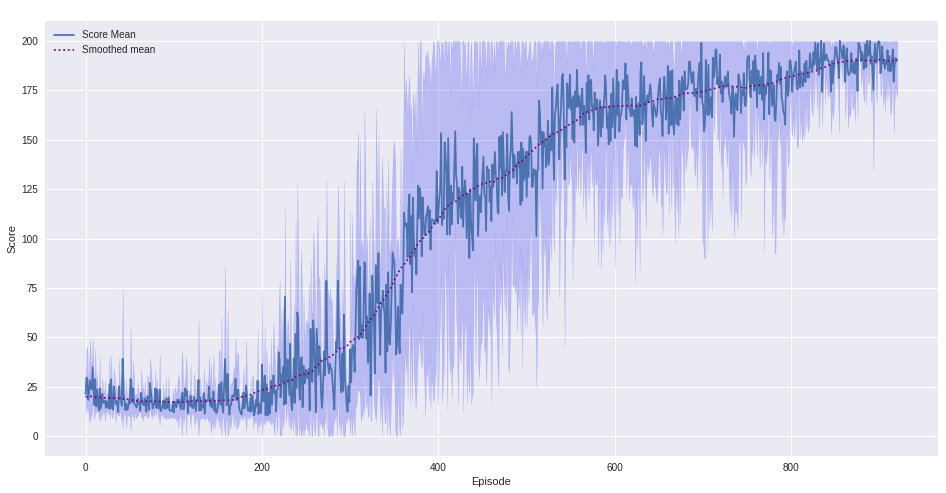
\includegraphics[width=\linewidth]{plot_score.png}
    \caption{Final results: plot of the obtained averaged out of a pool of 6 training runs. The light blue lines represent the confidence interval obtained via mean $\pm$ standard deviation. Most of the runs are able to get to the desired score in $\sim$ 800 episodes}
    \label{fig:results}
\end{figure}
As shown in Figure \ref{fig:results}, the inverted pendulum system is able to stabilize to obtain the 200 score. As to the best of the author's knowledge, this result has not been obtained yet in the Cartpole-v0 environment with DQN and only raw visual input, mainly because of the absence of early stopping which prevents overfitting.\\

% \footnote{The algorithm can be found at this \href{https://github.com/fedebberto/Vision_Based_CartPole_DQN}{Federico Berto's Github repository}.}

\section{Potential Improvements and Future Work}
Reinforcement Learning is fast-paced research area and it is even difficult at times to catch up with the latest trends. Regarding the control systems in particular, algorithms such as the LQR and MPCs still offer better performance and, most of all, theoretical guarantees on stability, at the cost of needing more information on the state and/or model of the system. \\
As we can also notice from the results, even though there is a confidence baseline for the stabilization score, the system is still prone to disturbances and inherent instabilities of the control policy and the neural network approximating the state-action values. One research direction would be to look for robust formulations of the problem \cite{DBLP:journals/corr/PintoDSG17}. Another interesting area, which has more technical guarantees on convergence and more efficient sampling of the state-space is the \textit{Model-Based} Reinforcement Learning \cite{DBLP:journals/corr/abs-1903-00374}, although it inherently needs a description via a model, thus renouncing the \textit{model-free} paradigm. Perhaps, the most interesting research direction is the combination of Reinforcement Learning and/or Optimal Control with Neural Ordinary Differential Equations \cite{NEURIPS2018_69386f6b}, a new class of Neural Networks which, thanks to their inherent capability to deal with differential equations, are revolutionizing the area of approximation and optimization of complex dynamical systems.

\section{Conclusion}
The goal of this report was to find a controller in a situation where state variables were not available, in particular by using only raw images to generate a control policy.
The test benchmark we used is the inverted pendulum, which is used frequently to test non-linear controllers, which we used by extracting the necessary state information automatically thanks to the Deep Q-Learning, a Deep Reinforcement Learning algorithm capable of controlling agents with complex state-action spaces.\\
After implementing several tweaks to existing algorithms, we were able to obtain a controller capable of successfully obtaining the maximum reward score in the simulation by using Convolutional Neural Networks for choosing the optimal action leading to the optimal cumulative reward. The successful stabilization of the inverted pendulum shows that Reinforcement Learning is indeed capable of achieving good performances even with diffucult tasks.\\
Possible future developments include the implementation of new frameworks, such as Neural Ordinary Differential Equations, possibly paving the way to a better synergy of Reinforcement Learning and Optimal Control.
\printbibliography
\end{document}